
%% bare_jrnl.tex
%% V1.3
%% 2007/01/11
%% by Michael Shell
%% see http://www.michaelshell.org/
%% for current contact information.
%%
%% This is a skeleton file demonstrating the use of IEEEtran.cls
%% (requires IEEEtran.cls version 1.7 or later) with an IEEE journal paper.
%%
%% Support sites:
%% http://www.michaelshell.org/tex/ieeetran/
%% http://www.ctan.org/tex-archive/macros/latex/contrib/IEEEtran/
%% and
%% http://www.ieee.org/



% *** Authors should verify (and, if needed, correct) their LaTeX system  ***
% *** with the testflow diagnostic prior to trusting their LaTeX platform ***
% *** with production work. IEEE's font choices can trigger bugs that do  ***
% *** not appear when using other class files.                            ***
% The testflow support page is at:
% http://www.michaelshell.org/tex/testflow/


%%*************************************************************************
%% Legal Notice:
%% This code is offered as-is without any warranty either expressed or
%% implied; without even the implied warranty of MERCHANTABILITY or
%% FITNESS FOR A PARTICULAR PURPOSE! 
%% User assumes all risk.
%% In no event shall IEEE or any contributor to this code be liable for
%% any damages or losses, including, but not limited to, incidental,
%% consequential, or any other damages, resulting from the use or misuse
%% of any information contained here.
%%
%% All comments are the opinions of their respective authors and are not
%% necessarily endorsed by the IEEE.
%%
%% This work is distributed under the LaTeX Project Public License (LPPL)
%% ( http://www.latex-project.org/ ) version 1.3, and may be freely used,
%% distributed and modified. A copy of the LPPL, version 1.3, is included
%% in the base LaTeX documentation of all distributions of LaTeX released
%% 2003/12/01 or later.
%% Retain all contribution notices and credits.
%% ** Modified files should be clearly indicated as such, including  **
%% ** renaming them and changing author support contact information. **
%%
%% File list of work: IEEEtran.cls, IEEEtran_HOWTO.pdf, bare_adv.tex,
%%                    bare_conf.tex, bare_jrnl.tex, bare_jrnl_compsoc.tex
%%*************************************************************************

% Note that the a4paper option is mainly intended so that authors in
% countries using A4 can easily print to A4 and see how their papers will
% look in print - the typesetting of the document will not typically be
% affected with changes in paper size (but the bottom and side margins will).
% Use the testflow package mentioned above to verify correct handling of
% both paper sizes by the user's LaTeX system.
%
% Also note that the "draftcls" or "draftclsnofoot", not "draft", option
% should be used if it is desired that the figures are to be displayed in
% draft mode.
%
\documentclass[journal]{IEEEtran}
%
% If IEEEtran.cls has not been installed into the LaTeX system files,
% manually specify the path to it like:
% \documentclass[journal]{../sty/IEEEtran}

\bibliographystyle{IEEEtran}

\usepackage{algorithm2e}
\usepackage{empheq}


% Some very useful LaTeX packages include:
% (uncomment the ones you want to load)


% *** MISC UTILITY PACKAGES ***
%
%\usepackage{ifpdf}
% Heiko Oberdiek's ifpdf.sty is very useful if you need conditional
% compilation based on whether the output is pdf or dvi.
% usage:
% \ifpdf
%   % pdf code
% \else
%   % dvi code
% \fi
% The latest version of ifpdf.sty can be obtained from:
% http://www.ctan.org/tex-archive/macros/latex/contrib/oberdiek/
% Also, note that IEEEtran.cls V1.7 and later provides a builtin
% \ifCLASSINFOpdf conditional that works the same way.
% When switching from latex to pdflatex and vice-versa, the compiler may
% have to be run twice to clear warning/error messages.






% *** CITATION PACKAGES ***
%
%\usepackage{cite}
% cite.sty was written by Donald Arseneau
% V1.6 and later of IEEEtran pre-defines the format of the cite.sty package
% \cite{} output to follow that of IEEE. Loading the cite package will
% result in citation numbers being automatically sorted and properly
% "compressed/ranged". e.g., [1], [9], [2], [7], [5], [6] without using
% cite.sty will become [1], [2], [5]--[7], [9] using cite.sty. cite.sty's
% \cite will automatically add leading space, if needed. Use cite.sty's
% noadjust option (cite.sty V3.8 and later) if you want to turn this off.
% cite.sty is already installed on most LaTeX systems. Be sure and use
% version 4.0 (2003-05-27) and later if using hyperref.sty. cite.sty does
% not currently provide for hyperlinked citations.
% The latest version can be obtained at:
% http://www.ctan.org/tex-archive/macros/latex/contrib/cite/
% The documentation is contained in the cite.sty file itself.






% *** GRAPHICS RELATED PACKAGES ***
%
\ifCLASSINFOpdf
  \usepackage[pdftex]{graphicx}
  % declare the path(s) where your graphic files are
  \graphicspath{{.}}
  % and their extensions so you won't have to specify these with
  % every instance of \includegraphics
  \DeclareGraphicsExtensions{.pdf,.jpeg,.png}
\else
  % or other class option (dvipsone, dvipdf, if not using dvips). graphicx
  % will default to the driver specified in the system graphics.cfg if no
  % driver is specified.
  % \usepackage[dvips]{graphicx}
  % declare the path(s) where your graphic files are
  % \graphicspath{{../eps/}}
  % and their extensions so you won't have to specify these with
  % every instance of \includegraphics
  % \DeclareGraphicsExtensions{.eps}
\fi
% graphicx was written by David Carlisle and Sebastian Rahtz. It is
% required if you want graphics, photos, etc. graphicx.sty is already
% installed on most LaTeX systems. The latest version and documentation can
% be obtained at: 
% http://www.ctan.org/tex-archive/macros/latex/required/graphics/
% Another good source of documentation is "Using Imported Graphics in
% LaTeX2e" by Keith Reckdahl which can be found as epslatex.ps or
% epslatex.pdf at: http://www.ctan.org/tex-archive/info/
%
% latex, and pdflatex in dvi mode, support graphics in encapsulated
% postscript (.eps) format. pdflatex in pdf mode supports graphics
% in .pdf, .jpeg, .png and .mps (metapost) formats. Users should ensure
% that all non-photo figures use a vector format (.eps, .pdf, .mps) and
% not a bitmapped formats (.jpeg, .png). IEEE frowns on bitmapped formats
% which can result in "jaggedy"/blurry rendering of lines and letters as
% well as large increases in file sizes.
%
% You can find documentation about the pdfTeX application at:
% http://www.tug.org/applications/pdftex





% *** MATH PACKAGES ***
%
%\usepackage[cmex10]{amsmath}
% A popular package from the American Mathematical Society that provides
% many useful and powerful commands for dealing with mathematics. If using
% it, be sure to load this package with the cmex10 option to ensure that
% only type 1 fonts will utilized at all point sizes. Without this option,
% it is possible that some math symbols, particularly those within
% footnotes, will be rendered in bitmap form which will result in a
% document that can not be IEEE Xplore compliant!
%
% Also, note that the amsmath package sets \interdisplaylinepenalty to 10000
% thus preventing page breaks from occurring within multiline equations. Use:
%\interdisplaylinepenalty=2500
% after loading amsmath to restore such page breaks as IEEEtran.cls normally
% does. amsmath.sty is already installed on most LaTeX systems. The latest
% version and documentation can be obtained at:
% http://www.ctan.org/tex-archive/macros/latex/required/amslatex/math/





% *** SPECIALIZED LIST PACKAGES ***
%
%\usepackage{algorithmic}
% algorithmic.sty was written by Peter Williams and Rogerio Brito.
% This package provides an algorithmic environment fo describing algorithms.
% You can use the algorithmic environment in-text or within a figure
% environment to provide for a floating algorithm. Do NOT use the algorithm
% floating environment provided by algorithm.sty (by the same authors) or
% algorithm2e.sty (by Christophe Fiorio) as IEEE does not use dedicated
% algorithm float types and packages that provide these will not provide
% correct IEEE style captions. The latest version and documentation of
% algorithmic.sty can be obtained at:
% http://www.ctan.org/tex-archive/macros/latex/contrib/algorithms/
% There is also a support site at:
% http://algorithms.berlios.de/index.html
% Also of interest may be the (relatively newer and more customizable)
% algorithmicx.sty package by Szasz Janos:
% http://www.ctan.org/tex-archive/macros/latex/contrib/algorithmicx/




% *** ALIGNMENT PACKAGES ***
%
%\usepackage{array}
% Frank Mittelbach's and David Carlisle's array.sty patches and improves
% the standard LaTeX2e array and tabular environments to provide better
% appearance and additional user controls. As the default LaTeX2e table
% generation code is lacking to the point of almost being broken with
% respect to the quality of the end results, all users are strongly
% advised to use an enhanced (at the very least that provided by array.sty)
% set of table tools. array.sty is already installed on most systems. The
% latest version and documentation can be obtained at:
% http://www.ctan.org/tex-archive/macros/latex/required/tools/


%\usepackage{mdwmath}
%\usepackage{mdwtab}
% Also highly recommended is Mark Wooding's extremely powerful MDW tools,
% especially mdwmath.sty and mdwtab.sty which are used to format equations
% and tables, respectively. The MDWtools set is already installed on most
% LaTeX systems. The lastest version and documentation is available at:
% http://www.ctan.org/tex-archive/macros/latex/contrib/mdwtools/


% IEEEtran contains the IEEEeqnarray family of commands that can be used to
% generate multiline equations as well as matrices, tables, etc., of high
% quality.


%\usepackage{eqparbox}
% Also of notable interest is Scott Pakin's eqparbox package for creating
% (automatically sized) equal width boxes - aka "natural width parboxes".
% Available at:
% http://www.ctan.org/tex-archive/macros/latex/contrib/eqparbox/





% *** SUBFIGURE PACKAGES ***
%\usepackage[tight,footnotesize]{subfigure}
% subfigure.sty was written by Steven Douglas Cochran. This package makes it
% easy to put subfigures in your figures. e.g., "Figure 1a and 1b". For IEEE
% work, it is a good idea to load it with the tight package option to reduce
% the amount of white space around the subfigures. subfigure.sty is already
% installed on most LaTeX systems. The latest version and documentation can
% be obtained at:
% http://www.ctan.org/tex-archive/obsolete/macros/latex/contrib/subfigure/
% subfigure.sty has been superceeded by subfig.sty.



%\usepackage[caption=false]{caption}
%\usepackage[font=footnotesize]{subfig}
% subfig.sty, also written by Steven Douglas Cochran, is the modern
% replacement for subfigure.sty. However, subfig.sty requires and
% automatically loads Axel Sommerfeldt's caption.sty which will override
% IEEEtran.cls handling of captions and this will result in nonIEEE style
% figure/table captions. To prevent this problem, be sure and preload
% caption.sty with its "caption=false" package option. This is will preserve
% IEEEtran.cls handing of captions. Version 1.3 (2005/06/28) and later 
% (recommended due to many improvements over 1.2) of subfig.sty supports
% the caption=false option directly:
%\usepackage[caption=false,font=footnotesize]{subfig}
%
% The latest version and documentation can be obtained at:
% http://www.ctan.org/tex-archive/macros/latex/contrib/subfig/
% The latest version and documentation of caption.sty can be obtained at:
% http://www.ctan.org/tex-archive/macros/latex/contrib/caption/




% *** FLOAT PACKAGES ***
%
%\usepackage{fixltx2e}
% fixltx2e, the successor to the earlier fix2col.sty, was written by
% Frank Mittelbach and David Carlisle. This package corrects a few problems
% in the LaTeX2e kernel, the most notable of which is that in current
% LaTeX2e releases, the ordering of single and double column floats is not
% guaranteed to be preserved. Thus, an unpatched LaTeX2e can allow a
% single column figure to be placed prior to an earlier double column
% figure. The latest version and documentation can be found at:
% http://www.ctan.org/tex-archive/macros/latex/base/



%\usepackage{stfloats}
% stfloats.sty was written by Sigitas Tolusis. This package gives LaTeX2e
% the ability to do double column floats at the bottom of the page as well
% as the top. (e.g., "\begin{figure*}[!b]" is not normally possible in
% LaTeX2e). It also provides a command:
%\fnbelowfloat
% to enable the placement of footnotes below bottom floats (the standard
% LaTeX2e kernel puts them above bottom floats). This is an invasive package
% which rewrites many portions of the LaTeX2e float routines. It may not work
% with other packages that modify the LaTeX2e float routines. The latest
% version and documentation can be obtained at:
% http://www.ctan.org/tex-archive/macros/latex/contrib/sttools/
% Documentation is contained in the stfloats.sty comments as well as in the
% presfull.pdf file. Do not use the stfloats baselinefloat ability as IEEE
% does not allow \baselineskip to stretch. Authors submitting work to the
% IEEE should note that IEEE rarely uses double column equations and
% that authors should try to avoid such use. Do not be tempted to use the
% cuted.sty or midfloat.sty packages (also by Sigitas Tolusis) as IEEE does
% not format its papers in such ways.


%\ifCLASSOPTIONcaptionsoff
%  \usepackage[nomarkers]{endfloat}
% \let\MYoriglatexcaption\caption
% \renewcommand{\caption}[2][\relax]{\MYoriglatexcaption[#2]{#2}}
%\fi
% endfloat.sty was written by James Darrell McCauley and Jeff Goldberg.
% This package may be useful when used in conjunction with IEEEtran.cls'
% captionsoff option. Some IEEE journals/societies require that submissions
% have lists of figures/tables at the end of the paper and that
% figures/tables without any captions are placed on a page by themselves at
% the end of the document. If needed, the draftcls IEEEtran class option or
% \CLASSINPUTbaselinestretch interface can be used to increase the line
% spacing as well. Be sure and use the nomarkers option of endfloat to
% prevent endfloat from "marking" where the figures would have been placed
% in the text. The two hack lines of code above are a slight modification of
% that suggested by in the endfloat docs (section 8.3.1) to ensure that
% the full captions always appear in the list of figures/tables - even if
% the user used the short optional argument of \caption[]{}.
% IEEE papers do not typically make use of \caption[]'s optional argument,
% so this should not be an issue. A similar trick can be used to disable
% captions of packages such as subfig.sty that lack options to turn off
% the subcaptions:
% For subfig.sty:
% \let\MYorigsubfloat\subfloat
% \renewcommand{\subfloat}[2][\relax]{\MYorigsubfloat[]{#2}}
% For subfigure.sty:
% \let\MYorigsubfigure\subfigure
% \renewcommand{\subfigure}[2][\relax]{\MYorigsubfigure[]{#2}}
% However, the above trick will not work if both optional arguments of
% the \subfloat/subfig command are used. Furthermore, there needs to be a
% description of each subfigure *somewhere* and endfloat does not add
% subfigure captions to its list of figures. Thus, the best approach is to
% avoid the use of subfigure captions (many IEEE journals avoid them anyway)
% and instead reference/explain all the subfigures within the main caption.
% The latest version of endfloat.sty and its documentation can obtained at:
% http://www.ctan.org/tex-archive/macros/latex/contrib/endfloat/
%
% The IEEEtran \ifCLASSOPTIONcaptionsoff conditional can also be used
% later in the document, say, to conditionally put the References on a 
% page by themselves.





% *** PDF, URL AND HYPERLINK PACKAGES ***
%
%\usepackage{url}
% url.sty was written by Donald Arseneau. It provides better support for
% handling and breaking URLs. url.sty is already installed on most LaTeX
% systems. The latest version can be obtained at:
% http://www.ctan.org/tex-archive/macros/latex/contrib/misc/
% Read the url.sty source comments for usage information. Basically,
% \url{my_url_here}.





% *** Do not adjust lengths that control margins, column widths, etc. ***
% *** Do not use packages that alter fonts (such as pslatex).         ***
% There should be no need to do such things with IEEEtran.cls V1.6 and later.
% (Unless specifically asked to do so by the journal or conference you plan
% to submit to, of course. )


% correct bad hyphenation here
\hyphenation{op-tical net-works semi-conduc-tor}


\begin{document}
%
% paper title
% can use linebreaks \\ within to get better formatting as desired
\title{Side channel attacks over ECC: Review}
%
%
% author names and IEEE memberships
% note positions of commas and nonbreaking spaces ( ~ ) LaTeX will not break
% a structure at a ~ so this keeps an author's name from being broken across
% two lines.
% use \thanks{} to gain access to the first footnote area
% a separate \thanks must be used for each paragraph as LaTeX2e's \thanks
% was not built to handle multiple paragraphs
%

\author{Franck~de~Goer~%,~\IEEEmembership{Member,~IEEE,}
        and~Guillaume~Jeanne%,~\IEEEmembership{Life~Fellow,~IEEE}% <-this % stops a space
%\thanks{M. Shell is with the Department
%of Electrical and Computer Engineering, Georgia Institute of Technology, Atlanta,
%GA, 30332 USA e-mail: (see http://www.michaelshell.org/contact.html).}% <-this % stops a space
%\thanks{J. Doe and J. Doe are with Anonymous University.}% <-this % stops a space
%\thanks{Manuscript received April 19, 2005; revised January 11, 2007.}
}

% note the % following the last \IEEEmembership and also \thanks - 
% these prevent an unwanted space from occurring between the last author name
% and the end of the author line. i.e., if you had this:
% 
% \author{....lastname \thanks{...} \thanks{...} }
%                     ^------------^------------^----Do not want these spaces!
%
% a space would be appended to the last name and could cause every name on that
% line to be shifted left slightly. This is one of those "LaTeX things". For
% instance, "\textbf{A} \textbf{B}" will typeset as "A B" not "AB". To get
% "AB" then you have to do: "\textbf{A}\textbf{B}"
% \thanks is no different in this regard, so shield the last } of each \thanks
% that ends a line with a % and do not let a space in before the next \thanks.
% Spaces after \IEEEmembership other than the last one are OK (and needed) as
% you are supposed to have spaces between the names. For what it is worth,
% this is a minor point as most people would not even notice if the said evil
% space somehow managed to creep in.



% The paper headers
\markboth{Advanced Cryptography, January 2014}
{Shell \MakeLowercase{\textit{et al.}}: Bare Demo of IEEEtran.cls for Journals}
% The only time the second header will appear is for the odd numbered pages
% after the title page when using the twoside option.
% 
% *** Note that you probably will NOT want to include the author's ***
% *** name in the headers of peer review papers.                   ***
% You can use \ifCLASSOPTIONpeerreview for conditional compilation here if
% you desire.




% If you want to put a publisher's ID mark on the page you can do it like
% this:
%\IEEEpubid{0000--0000/00\$00.00~\copyright~2007 IEEE}
% Remember, if you use this you must call \IEEEpubidadjcol in the second
% column for its text to clear the IEEEpubid mark.



% use for special paper notices
%\IEEEspecialpapernotice{(Invited Paper)}




% make the title area
\maketitle


\begin{abstract}
%\boldmath
In this article, we will explain what a side-channel attack is and how it can be a threat to elliptic curves cryptography. We have decided to make an overview of different methods and only detail a few of them that have an important impact on elliptic curves cryptography. For each attack, we propose several methods to prevent these attacks or to minimize the impact on cryptanalysis.

\end{abstract}
% IEEEtran.cls defaults to using nonbold math in the Abstract.
% This preserves the distinction between vectors and scalars. However,
% if the journal you are submitting to favors bold math in the abstract,
% then you can use LaTeX's standard command \boldmath at the very start
% of the abstract to achieve this. Many IEEE journals frown on math
% in the abstract anyway.

% Note that keywords are not normally used for peerreview papers.
\begin{IEEEkeywords}
ECC, Side channel attacks, Timing attack, Power consumption attack, DPA, double and add.
\end{IEEEkeywords}






% For peer review papers, you can put extra information on the cover
% page as needed:
% \ifCLASSOPTIONpeerreview
% \begin{center} \bfseries EDICS Category: 3-BBND \end{center}
% \fi
%
% For peerreview papers, this IEEEtran command inserts a page break and
% creates the second title. It will be ignored for other modes.
\IEEEpeerreviewmaketitle



\section{Introduction}

\IEEEPARstart{S}{ide-channel} attacks take advantage of the interaction between a module and its environment when it uses sensitive data. Most of the time, it applies to the embedded world, such as smart cards which are frequently used with cryptography to authenticate a user. Such channel can be measurement of the time, power analysis, electro-magnetic analysis or acoustic analysis.\\

These channels will allow us to find some secret information because of two main points. We can have software or hardware leaks. Software leaks are due to branching condition in algorithms. Depending on the branch taken by the program, operations will not be the same. With these channels, we are able to detect what branch was taken. Second point is hardware leaks, each operation made by the processor consumes an amount of power which depends on the hamming weight of the value of manipulated data.\\

This issue is at the heart of embedded security, a lot of research papers are published every month and attacks are more and more sophisticated. Last month, Daniel Genkin, Adi Shamir and Eran Tromer published a paper entitled 
{\it RSA Key Extraction via Low-Bandwidth Acoustic Cryptanalysis} (see \cite{genkin2013rsa}) where they showed that they can retrieve a RSA key using a standard microphone to listen the noise emitted by a processor.\\

In this article, we will present several side-channel attacks and apply them to elliptic curve cryptanalysis. Then, we will show how we can protect ourselves from these attacks.\\

The main support for this article was the "Handbook of elliptic and hyper-elliptic curve cryptography" \cite{cohen2010handbook}.



% needed in second column of first page if using \IEEEpubid
%\IEEEpubidadjcol



% An example of a floating figure using the graphicx package.
% Note that \label must occur AFTER (or within) \caption.
% For figures, \caption should occur after the \includegraphics.
% Note that IEEEtran v1.7 and later has special internal code that
% is designed to preserve the operation of \label within \caption
% even when the captionsoff option is in effect. However, because
% of issues like this, it may be the safest practice to put all your
% \label just after \caption rather than within \caption{}.
%
% Reminder: the "draftcls" or "draftclsnofoot", not "draft", class
% option should be used if it is desired that the figures are to be
% displayed while in draft mode.
%
%\begin{figure}[!t]
%\centering
%\includegraphics[width=2.5in]{myfigure}
% where an .eps filename suffix will be assumed under latex, 
% and a .pdf suffix will be assumed for pdflatex; or what has been declared
% via \DeclareGraphicsExtensions.
%\caption{Simulation Results}
%\label{fig_sim}
%\end{figure}

% Note that IEEE typically puts floats only at the top, even when this
% results in a large percentage of a column being occupied by floats.


% An example of a double column floating figure using two subfigures.
% (The subfig.sty package must be loaded for this to work.)
% The subfigure \label commands are set within each subfloat command, the
% \label for the overall figure must come after \caption.
% \hfil must be used as a separator to get equal spacing.
% The subfigure.sty package works much the same way, except \subfigure is
% used instead of \subfloat.
%
%\begin{figure*}[!t]
%\centerline{\subfloat[Case I]\includegraphics[width=2.5in]{subfigcase1}%
%\label{fig_first_case}}
%\hfil
%\subfloat[Case II]{\includegraphics[width=2.5in]{subfigcase2}%
%\label{fig_second_case}}}
%\caption{Simulation results}
%\label{fig_sim}
%\end{figure*}
%
% Note that often IEEE papers with subfigures do not employ subfigure
% captions (using the optional argument to \subfloat), but instead will
% reference/describe all of them (a), (b), etc., within the main caption.


% An example of a floating table. Note that, for IEEE style tables, the 
% \caption command should come BEFORE the table. Table text will default to
% \footnotesize as IEEE normally uses this smaller font for tables.
% The \label must come after \caption as always.
%
%\begin{table}[!t]
%% increase table row spacing, adjust to taste
%\renewcommand{\arraystretch}{1.3}
% if using array.sty, it might be a good idea to tweak the value of
% \extrarowheight as needed to properly center the text within the cells
%\caption{An Example of a Table}
%\label{table_example}
%\centering
%% Some packages, such as MDW tools, offer better commands for making tables
%% than the plain LaTeX2e tabular which is used here.
%\begin{tabular}{|c||c|}
%\hline
%One & Two\\
%\hline
%Three & Four\\
%\hline
%\end{tabular}
%\end{table}


% Note that IEEE does not put floats in the very first column - or typically
% anywhere on the first page for that matter. Also, in-text middle ("here")
% positioning is not used. Most IEEE journals use top floats exclusively.
% Note that, LaTeX2e, unlike IEEE journals, places footnotes above bottom
% floats. This can be corrected via the \fnbelowfloat command of the
% stfloats package.


\section{The sensible point: double and add}

{\it From this point, we will focus until the end of the paper on vulnerabilities on the "double and add" algorithm. 
In this section, we will explain why it is interesting to study this particular algorithm, and also why it is the main sensitive point
of elliptic curve cryptography algorithms.}

\subsection{The double-and-add algorithm}

\subsubsection{Principle}
The "double and add" algorithm is a very useful algorithm in {\tt ECC}, because it is used to compute the scalar multiplication on elliptic curve ; 
exactly in the same way that modular exponentiation is central in most of arithmetic cryptography schemes. 
A lot of {\tt ECC} schemes are based on the discrete logarithm problem (DLP) over a cyclic group generated by a point on an elliptic curve.
For a given scalar $d$ and a point $P$ on an elliptic curve, it is assumed to be hard to retrieve the value of $d$ from the point $[d]P$. 
The attacks described in the next sections of this paper aim to retrieve the value of $d$, either by performing measures (on the time of computation, 
the power consumption, etc.) or by introducing errors during the computation of $[d]P$.
More on genericity of those two algorithms 
in section \ref{genericity}.\\

\subsubsection{Algorithm}
\label{sensible-point-algo}
The basic algorithm for double-and-add is given in Algorithm \ref{d-and-a-algo}.

\begin{algorithm}
%    \SetLine % For v3.9
    \SetAlgoLined % For previous releases [?]
   
    \SetKwComment{tcc}{/* }{ */}
    \SetSideCommentLeft 
    \SetNoFillComment

    \KwData{P: base point ; d: scalar}
    
    \KwResult{Q = [d]P resulting point}
    
    Q $\leftarrow$ 0\;
    l $\leftarrow$ $log_2(d)$\;
    \For{i from l downto 0}{
        \tcc{Using point doubling}
        Q $\leftarrow$ [2]Q\; 
        \If{d[i] == 1}{
            \tcc{Using point adding}
            Q $\leftarrow$ Q + P\; 
        }
    }
    \Return{Q}

    \bigskip

    \caption{Basic Double-and-Add algorithm}
    \label{d-and-a-algo}

\end{algorithm}

\subsection{Genericity of the modular exponentiation and the double-and-add algorithm}
\label{genericity}
For many classical cryptographic schemes, 
at some point we will need to compute $x^k mod p$, where (usually) $k$ is related to the secret key (or the private key). For instance, in {\tt RSA}, 
the signature of a message $m$ with a private key $(N, e)$ is the following: 
$$ c = m^e~mod~N $$

With {\tt El Gamal}, the encryption scheme also includes a step of modular exponentiation with a secret element:
$$ s = h^y~mod~q$$
where $y$ is a random integer in $\{1, .., q-1\}$. The knowledge of $y$ leads to the knowledge of the plain-text without need of the private key. 
More details in appendix \ref{ElGamal}.\\

In both cases we can see that a weakness on the modular exponentiation that allows to deduce the exponent would lead to an attack.
In the same way, the double-and-add algorithm is used in every scheme based on elliptic curves, and if it leaks information about the 
scalar element, then a lot of classical algorithms can be attacked. For example, consider the {\tt ECIES} algorithm to cipher/decipher messages. 
The algorithm is given in Algorithm \ref{ecies-decrypt}. We can see at line 1 that the private key is used in a double-and-add function to compute
$[k]P$. 

\begin{algorithm}

    \SetAlgoLined

    \SetKwComment{tcc}{/* }{ */}
    \SetSideCommentLeft 
    \SetNoFillComment

    \LinesNumbered

    \KwData{(R, c, d): cipher-text, EC: elliptic curve, P: base point, n: order of P, k: private key, E: symmetric encryption scheme, MAC: message authentication code function, KDF: key derivation function}
    \KwResult{m: message}
    
    (x, y) $\leftarrow$ [k]R\;
    \If{x == 0 and y == 0}{
        \Return{Failure}\;
    }

    \tcc{Key derivation}
    $k_e||k_m$ $\leftarrow$ KDF(x)\;
    
    \If{d != MAC($k_m$, c)}{
        \Return{Failure}\;
    }

    \tcc{Decryption of the symmetric cipher}
    m = $E^{-1}$($k_e$, c)\;

    \Return{m}

    \caption{Decipher c in ECIES}
    \label{ecies-decrypt}

\end{algorithm}


% ECDSA algorithm - useless at this point
%\begin{algorithm}
%    
%    \SetAlgoLined
%
%    \SetKwComment{tcc}{/* }{ */}
%    \SetSideCommentLeft 
%    \SetNoFillComment
%
%    \LinesNumbered 
%
%    \KwData{m: message to sign, C: elliptic curve, P: base point, n: order of P, $d_A$: private key}
%    
%    \KwResult{S: signature of m}
%
%    e $\leftarrow$ Hash(m)\;
%    l $\leftarrow$ $log_2(n)$\;
%    z $\leftarrow$ e[1:n]\;
%    k $\leftarrow$ random(1, n-1)\;
%    (x, y) $\leftarrow$ [k]P\;
%    r $\leftarrow$ x mod n\;
%    \If{r == 0}{
%        go back to line 4\; 
%    }
%    s $\leftarrow$ $k^{-1}*(z + r*d_A)~mod~n$\;
%    \Return{(r, s)}
%    
%\end{algorithm}


We will see in next sections what side-channel attacks can be performed on this naive version, 
and the possible counter-measures that lead to a more robust implementation. Section \ref{non-intrusive}
deals with non-intrusive attacks, such as timing attacks and power analysis attacks. Section~\ref{fault}
deals with fault attacks.



\section{Non-intrusive attacks}
\label{non-intrusive}  

Non-intrusive attacks are attacks which do not destroy or alter the functioning of the device. Besides they cannot be detected by the user of the card. 
   
    \subsection{Timing attacks}

Timing attack was the first side-channel attack and one of the simplest. It consists in measuring the time dedicated to the computation of an algorithm. With this time, we can deduce how many times the program runs into a given loop.
To protect against these attacks, implementations of an algorithm have to do the same number of loop, whatever the input of the loop condition is. \\

Today, timing attacks are no longer considered because power analysis attacks are more efficient and as simple to set up. Almost no timing attacks against ECC have been published.

    \subsection{Power analysis attacks}

The goal is to measure the power consumption of the device while it is running the program. To set up these attacks, we need an oscilloscope and a card reader.
Two methods are used to extract the key, the simple power analysis (SPA) and the differential power analysis (DPA). We will go further these two methods.\\

        \subsubsection{SPA}
With simple power analysis, we just need one curve corresponding to one measurement of the consumption. From this curve, we can guess the secret key because each operation does not have the same power consumption. For instance with elliptic curve, the point adding is more expensive than the point doubling. In the basic double-and-add algorithm, we can know at each step if the addition is computed, if it is the case then we know that $ d[i]==1 $. At the end we are able to know the entire private key. Besides, an attacker can recognize point doubling from point adding because point adding cannot occurs twice at the time, it is only possible for point doubling.

\begin{figure}[h]
   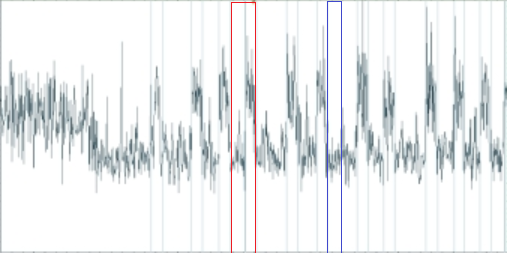
\includegraphics[scale=0.65]{spa.png}
   \caption{\label{spa.png} SPA against double-and-add from an IPod touch.}
\end{figure}

In figure \ref{spa.png}, we can see the consumption curve for a double-and-add using elliptic curve on a IPod touch. On this curve, each peak corresponds to a add operation. As we have said before, this operation is more expensive than the point doubling. Point doubling is represented in the blue rectangle. Then in the red one, we can observe a round of the loop where there is both operations: point doubling and point adding. Then the red rectangle corresponds to a bit equals to 1 and the blue to a bit equals to 0. This is coherent with the fact that we cannot have twice add at the time. From this, we can deduce the key, which is in binary 111011011011101 ($=30429$). Please remark that if the double-and-add is performed from right to left instead of left to right, we have to read the graph from right to left to obtain the key.

\begin{algorithm}
%    \SetLine % For v3.9
    \SetAlgoLined % For previous releases [?]
   
    \SetKwComment{tcc}{/* }{ */}
    \SetSideCommentLeft 
    \SetNoFillComment

    \KwData{P: base point ; d: scalar}
    
    \KwResult{Q = [d]P resulting point}
    
    Q $\leftarrow$ 0\;
    R $\leftarrow$ 0\;
    l $\leftarrow$ $log_2(d)$\;
    \For{i from l downto 0}{
        \tcc{Using point doubling}
        Q $\leftarrow$ [2]Q\; 
        \If{d[i] == 1}{
            \tcc{Using point adding}
            Q $\leftarrow$ Q + P\; 
        } \Else {
	    \tcc{R is not used}
	    R $\leftarrow$ Q + P\; 
	}
    }
    \Return{Q}

    \bigskip

    \caption{Resistant Double-and-Add algorithm}
    \label{resistent-daa}
\end{algorithm}

To protect against SPA, that the algorithm has to always perform the same operations. We propose in algorithm \ref{resistent-daa} an implementation of the double-and-add robust against SPA.
As you can see, the addition is always performed but the result is not used when the corresponding bit is not equal to 1. Then at each step, the amount of power consumed is the same.\\

        \subsubsection{DPA}

SPA relies mainly on software leaks contrary to differential power analysis which exploit the hamming weight of manipulated data. DPA requires a lot of experiments, and acquisition of many power consumption curves. Usually we need several thousands of curves. The goal is to collect a lot of curves corresponding to encryption with different known messages at each step (but the same key). Then the attacker makes some assumptions about few bits of the key and he uses these to compute intermediate values of the encryption algorithm. Then the attacker sort the set of curves into two sets, according to the power consumption at the point where he computed intermediate values. By making the subtraction between the mean of each set, the attacker can know if his supposition was true or not. \\

To succeed with DPA, we need the key to be the same at each acquisition, which is not the case in randomized algorithms such as ECDSA or HECDSA. Nevertheless, some elliptic curve algorithms are vulnerable, such as El Gamal.\\

A countermeasure is to randomize intermediate values of the algorithm. For instance in elliptic curve, we can randomize the curve or the coordinates of the basis of calculation.
It is also possible to consider other curves, where formulas for addition are unified. This means that the same formula is valid both for doubling and adding. This is well explained in chapter 29.1.2 of \cite{cohen2010handbook}.\\

Some other countermeasures can be considered in hardware: 
one can try to change the power consumption model in order to make it depend less on the hamming weight of data or increase noise to prevent recognition from curves.
        
\section{Fault attacks}
\label{fault}

\subsection{Assumptions}
In this section, we will deal with fault attacks. We will assume that an attacker is able to change bits of the registers
during the computation. We will not discuss here if this fault model is relevant or not, but for further information, 
refer to \cite{bar2006sorcerer} or \cite{giraud2004survey}.

\subsection{Malicious input $P'$}
\label{malicious}
This attack is not, properly speaking, a fault attack as it is not needed to introduce any 
error during the computation. It relies, however, on the fact that a double-and-add algorithm 
do not check if the point $P$ given as an input is indeed a point on the elliptic curve $E$.
If it does not, we show that it is possible to reduce the DLP problem on the cyclic group of order $n$ on $E$ generated by $P$ to 
several DLPs of smaller cyclic groups of order $p_i | n$ on $E_i$ (still generated by $P$).
More details on this attack can be found in \cite{biehl2000differential} or \cite{cohen2010handbook}.\\

\subsubsection{Basic key}
\label{malicious-basic}
The main idea is to use the fact that the adding algorithm and the doubling algorithm do not depend on 
all the coefficients that define an elliptic curve (see Appendix \ref{adding-on-ec} for details).
Indeed, for a given curve $E = (a_1, a_2, a_3, a_4, a_6)$ over $K$, the addition of two points does not
depend on the value of $a_6$.\\

\subsubsection{Method} 
The first step is to find an elliptic curve $E' = (a_1, a_2, a_3, a_4, a_6')$ whose order is of the form
$$n' = \prod_{i = 0}^{k}p_i^{\alpha_i}$$
with $p_i$ small for all $i \in \{0, .., k\}$. As we pointed out in \ref{malicious-basic}, addition on $E$ is 
exactly the same as addition on $E'$, as the only coefficient that differs from $E$ to $E'$ is $a_6$. That means 
that if the double-and-add algorithm does not check if $P \in E$ before computing $[d]P$, then it is possible to 
give as an input $P_i \in E'$, of order $p_i$. The algorithm will compute $[d]P_i \in E'$, and then it leads to a DLP on a smaller 
group (of order $p_i$) that is easier to solve. By doing that with several $P_i$ of different orders $p_i$, and finally using 
the Chinese Reminder Theorem, it is possible to retrieve $d$.

\subsection{Fault injection at the beginning of the double-and-add}
Let $E = (a_1, a_2, a_3, a_4, a_6)$ be an elliptic curve over $K$.
We consider here that the algorithm check if the point given in input $P$ belongs
to the curve $E$ before starting the multiplication. If not, it returns {\tt failure}.\\

\subsubsection{Basic idea}
This attacks consists of giving a valid point $P$ as an input of the algorithm, and to 
inject a fault just after the verification. The result of the fault will be a change of the
stored value of $P$ to another value $P'$, which differs from $P$ by exactly one bit. 
However, the attacker is not able to know which bit was affected by the fault, so he 
does not know the point $P'$. \\

\subsubsection{Injection consequences}
With the fault injection, the algorithm will compute the value of $[d]P'$, with $P'$ very unlikely
belonging to $E$. We are in a very similar case to the attack described in \ref{malicious}, except that
there are some information missing. \\

\subsubsection{Getting back information}
At this point, we do not know $P'$, neither do we know the elliptic curve $E' = (a_1, a_2, a_3, a_4, a_6')$
such that $P' \in E'$. But using the output of the algorithm, we are able to recover these two pieces of information.
Indeed, if $P' \notin E$, then we can find $a_6'$ such that $P' \in E'$ with $E' = (a_1, a_2, a_3, a_4, a_6')$. $a_6'$ is uniquely determined by solving
the system given by $[d]P' \in E'$, where $[d]P'$ is known (it is the output of the algorithm), 
and all $a_i$ for $i \in \{1, .., 4\}$ are known. 
Once we know $E'$, we can find out $P'$ by testing all the points that differ of one bit from $P$, until we get a point that belongs to $E'$.
At this point, we have reduced the DLP in $E$ to a DLP on $E'$. \\

\subsubsection{Drawback}
This attack does not allow the attacker to choose $P'$ nor $E'$, so it relies on a part of luck to perform an attack
that leads to an easier DLP problem on $E'$ (in fact we need $E'$ to have a small divisor to be able to
get information about $d$). This attack will need several tries to recover the exact value of $d$.

\subsection{Fault injection during the double-and-add}
\label{attack-powa}
In this section, we will present an attack that allows the attacker to retrieve $d$ in polynomial time, by
introducing faults during the double-and-add computation. We will base the explanation on the algorithm given
in section \ref{sensible-point-algo} (Algorithm \ref{d-and-a-algo}). This attack is well described in \cite{biehl2000differential}.
Nevertheless, they use a right-to-left double-and-add algorithm, whereas the one that is used here is a left-to-right algorithm (see Algorithm \ref{d-and-a-algo}).
As explained in \ref{difficulties}, this leads to several new difficulties (as point halving).\\

\subsubsection{Notations}
We will use notations very similar to \cite{biehl2000differential}.
Let $d$ be the scalar, $n$ the length of $d$ in binary representation. We denote by $d[i]$ the $i^{th}$ bit of $d$, 
where $d[0]$ is the most significant bit of $d$. We also denote $d[a:b], 0 \leq a < b \leq n-1$ the concatenation of $d[i]$ for $i \in \{a, .., b\}$.
For example, $d = d[0:n-1]$.
We denote by $Q^{(i)}$ the state of the variable $Q$ before the $i^{th}$ iteration.\\

\subsubsection{Basic idea} 
After a first computation of $Q = [d]P$ for a given $P$ (in order to know the correct result of the scalar multiplication), the main idea 
is to introduce a one-bit fault during the $i^{th}$ iteration of the algorithm on $Q^{(i)}$, so that the end of the computation
will be performed starting from $Q'^{(i)}$. From the knowledge of $Q$ and $Q'$, the aim is to find $d[i:n-1]$ (to do this, we will also need 
to find out $Q'^{(i)}$).\\

\subsubsection{Finding out $Q'^{(i)}$ and $d[i:n-1]$}
At this point, we will try to find the first $i^* \in \{i, ..., n-1\}$ such that $d[i^*] = 1$. We will assume that there exist such a $i^*$ from now.
If at the end of the attack, we have found no good candidate, it will mean that such a $i^*$ does not exists, and then $d[i:n-1] = 0$.
To do this, we will iterate on all possible values of $j \in \{i, ..., n-1\}$ possible candidates for $i^*$, and on all possible $x \in \{0, 1\}^{n-1-j}$ 
possible candidates for $d[j:n-1]$, $n - j - 1$ least significant bits of d.
From each value of $j$ and $x$, we compute $Q_x^{(j)} = Q^{(n)} - [x]P$, candidate for $Q^{(i)}$. \\

\label{rq}
{\bf Remark.} This formula will only work if $i = 0$, that means that we are trying to compute the whole key at once. In other cases, it is more complicated
to find the first candidate for $Q^{(i)}$. This point is treated in \ref{difficulties}.\\


From $Q^{(i)}$ will be generated all possible values $Q'^{(i)}$ by flipping exactly one bit. To check if the values of $j$ and $x$ are correct, 
we will simulate the end of the computation from $Q'^{(i)}$ with the value of $x$ instead of $d[j:n-1]$ which is unknown. If the result of the computation
is equal to $Q'$, that means that the value of $x$ and $j$ are good candidates.
If there is only one good couple of candidates $(x, j)$, then it is the correct one, and we have then found the $n - 1 - i$ least significant bits of $d$ ($d[i:i*-1] = 0$ and $d[i*:n-1] = x$).
Otherwise, we need to redo the attack ; but one can show that the probability of having several good candidates is small 
(\cite{biehl2000differential}).\\

\subsubsection{Find out $d$}
\label{difficulties}
This section deals with the remark of section \ref{rq}.
In \cite{biehl2000differential}, the attack is at this point almost finished. Indeed, with a right-to-left algorithm, the key-bits are used from the LSB to the HSB. This means that 
once we have supposed a value for $x$ as a candidate for the $k$ HSB of $d$, we can reverse the end of the double-and-add computation by taking the final point 
$Q$ and subtracting $[2^{j}x]P$ (with $j = l - k$). This can be done without any knowledge about $d[j:n-1]$. Using this point, we can retrieve the key $d$ bit by bit, from $d[0]$ to 
$d[n-1]$ (using the HSB that are known to limit the space value for $x$).\\

Unfortunately, here, if we want to retrieve $d$ bit by bit (otherwise, the complexity of the attack is not polynomial), we will need to implement a point-halving algorithm. 
Indeed, as the double-and-add algorithm considered here is a left-from-right one, we need to retrieve the key from $d[n-1]$ to $d[0]$ (as explained previously). But to do that, we need
to be able to reverse several rounds of the double-and-add algorithm (to compute $Q_x^{(j)}$). And, in fact, without any knowledge on $d[0:j-1]$, we need to be able to perform point-halving
(see Algorithm \ref{rev-d-and-a-algo}). We propose a way to perform this in \ref{point-halving-sec}.
%If the value of $x$ is correct (meaning that it corresponds to the 
%$n - 1 - j$ least significant bits of $d$), then $

\begin{algorithm}
%    \SetLine % For v3.9
    \SetAlgoLined % For previous releases [?]
   
    \SetKwComment{tcc}{/* }{ */}
    \SetSideCommentLeft 
    \SetNoFillComment

    \KwData{Q = [d]P: resulting point, d: secret key, P: base point, k: number of iterations to reverse}
    
    \KwResult{R: intermediate point}
    
    R $\leftarrow$ Q\;
    l $\leftarrow$ $log_2(d)$\;
    \For{i from 0 downto k}{
        \If{d[l - i] == 1}{
            \tcc{Using point adding}
            R $\leftarrow$ R - P\; 
        }
        \tcc{POINT HALVING}
        R $\leftarrow$ Q/2\; 
    }
    \Return{R}

    \bigskip

    \caption{Basic Double-and-Add algorithm}
    \label{rev-d-and-a-algo}

\end{algorithm}

With this method, it is possible to deduce bit by bit the secret key $d$, even with a left-to-right double-and-add algorithm.\\

\subsubsection{Point halving}
\label{point-halving-sec}
\cite{rodriguezelliptic} describe a way to find out $P$ given $E$ and $[2]P$. We recall the main idea for a curve of the form $E: y^2 = x^3 + a_4x + a_6$ (which is the case of the curve we have chosen in \ref{implem}).
The goal is to reverse the function $elladd(E, P, P)$. From the formulas given in Appendix \ref{adding-on-ec}, if $P_1 = P_2 = P$, we have:

\begin{empheq}[left=\empheqlbrace]{align*}
    \lambda &= \frac{3 x_P^2 + 2 a_2 x_P + a_4 - a_1 y_P}{2 y_P - a_1 x_P - a_3} \\
    x_{[2]P} &= \lambda^2 + a_1 \lambda - a_2 - 2 x_P \\
    y_{[2]P} &= -y_P - (x_{[2]P} - x_P) \lambda - a_1 x_{[2]P} - a_3 
\end{empheq}

where the 3 unknown are $x_P, y_P$ and $\lambda$. For the simplified form, this gives:

\begin{empheq}[left=\empheqlbrace]{align*}
    \lambda &= \frac{3 x_P^2 + a_4}{2 y_P} \\ 
    x_{[2]P} &= \lambda^2 - 2 x_P  \\
    y_{[2]P} &= - y_P - (x_{[2]P} - x_P) \lambda
\end{empheq}

This leads to:

\begin{empheq}[left=\empheqlbrace]{align*}
    4 y_P^{2} x_{[2]P} = 9 x_P^{4} + 6 x_P^{2} a_{4} - 2 x_P + a_4^{2} \\
    y_P (2 y_{[2]P} + 1) = -(x_{[2]P} - x_P) (3 x_P^{2} + a_4) 
\end{empheq}

Now we can inject $y_P$ from the second equation to the first one. Then we obtain a univariate polynomial of degree 6 in $x_P$. Once you have $x_P$, you can deduce $y_P$ with the second equation. ($x_P$, $y_P$) is the point halving of R.


\section{Implementation}
\label{implem}
We propose here an implementation of the attack described in \ref{attack-powa} using {\tt Pari/GP}\footnote{See {\tt fault-attack.gp}}. The curve used is {\tt brainpoolP160r1} described in {\tt RFC5639}.

\subsection{Simulating fault injection}
To simulate fault injections, we add a parameter $k$ in the $double-and-add$ function, which indicates that we want to introduce a fault a iteration $k$. Then, at iteration $k$, the function will flip one random bit of
the abscissa of $Q$. The relevant code is the following: 

\begin{footnotesize}
\begin{verbatim}
if(i == k,
    b = random(floor(log(n)/log(2)) + 1);
    print("    ! Fault injection at iteration", k);
    Q = [Mod(bitxor(lift(Q[1]), (1<<b)), n), Q[2]];
);
\end{verbatim}
\end{footnotesize}

\subsection{Retrieving $d$ at once}
The first implementation only allowed to retrieve all the bits of $d$ at once, thus it was not a polynomial algorithm. The reason of this limitation is the problem described in \ref{difficulties}.
At this point, there is no call to a {\tt point-halving} algorithm, as $Q_x^{j} = P$.\\

\subsubsection{Problem encountered}
Except for the necessity of {\tt point-halving} already mentioned, two other complications came out during the implementation. The first one was the necessity of re-implementing {\tt elladd}, in 
order to be able to add two points that are not necessarily on the curve. Indeed, formulas given in Appendix \ref{adding-on-ec} have no reason to be limited to points on the curve. And as we are working with 
fault injections, at some point we are dealing with points that are "close" to points that are on the curve. And unfortunately, the basic version of {\tt elladd} checks if the points given in parameter belong to the curve.
To skip that, we implemented {\tt add\_point} that does not do the verification.\\ 

The second problem that was encountered was the subtraction operation. To do this, we had to implement a new function: {\tt neg\_point}, that takes a curve $E$ and a point $P$ as a parameter, and that returns a point that would be the
opposite of $P$ if $P$ is on the curve. Once again, we need the function to be able to do that on points that are not on the curve. The implementation uses the classical opposite formula on ECC: given $P = (x, y)$,
$$- P := (x, -y - a1*x - a3)$$

\subsubsection{Results}
The conclusion of this first implementation is that we are able to recover very small keys in a short time (within a few seconds for seven bits) with one fault injection at the first iteration.
Nevertheless, the computing time grows very fast as we add bits to the key size (see \ref{perf-all}).\\
Another interesting point is that we only have one candidate for $Q_x^{(j)}$ (as expected in \ref{rq}).

\begin{footnotesize}
\begin{verbatim}
$ gp fault-attack.gp 
[SECRET KEY] d = 107
[REFERENCE] Computing M = [d]P
[FAULT] Computing M' = ([d]P)' with fault injection
    ! Fault injection at iteration 1 !
[ATTACK] Retrieving d from M and M'
    ! Find out Q for d[1:7] = 107 !
\end{verbatim}
\end{footnotesize}

\subsubsection{Performance}
\label{perf-all}
As expected, the time for computing the attack is exponential in function of the length of the key $d$. Figure \ref{first-attack-perf} shows some results obtained for $d$ from $1$ to $255$. 
To obtain the graph, we have computed the average time of the attacks on every possible key of length $l$, for several values of $l$.

\begin{figure}
    \centering
    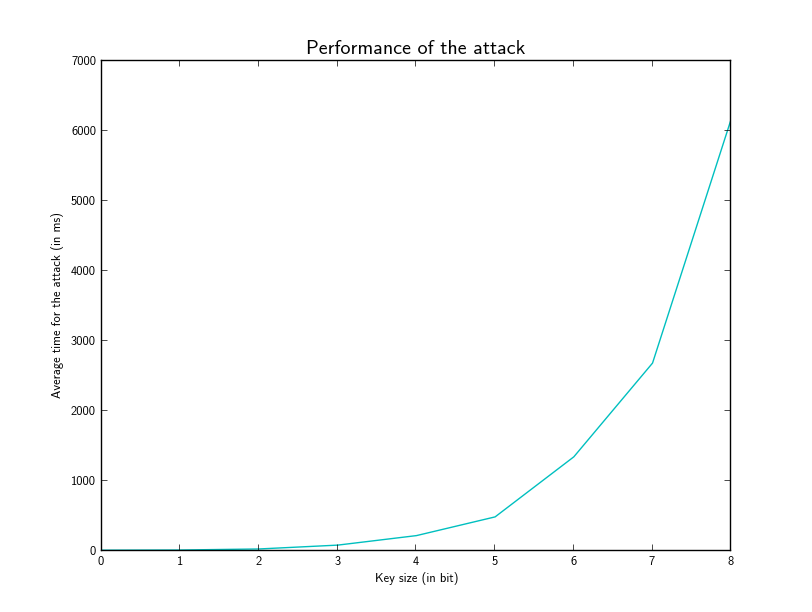
\includegraphics[width=250px]{img/first-attack-perf.png}
    \caption{Timing measures of the attack "at once" in function of the size of the key $d$}
    \label{first-attack-perf}
\end{figure}   


\subsection{Retrieving $d$ bit by bit}
As mentionned in section \ref{difficulties}, to be able to recover all bits of $d$ one by one, one need to be able to perform point-halving.
Unfortunately, we ran out of time, and were not be able to implement this point-halving, and thus not able to perform the bit-by-bit recovery.

\section{Conclusion}

In this article, we have seen some side-channel attacks and we applied them to elliptic curve cryptography. Some of these attacks are very simple to set up and do not damage the device. We saw that each countermeasure increase the cost of the algorithm. This can be a problem with an embedded device because they do not have a big computational power. The effectiveness of these attacks (and the counter-measures) depend on the hardware precision of the attacker. The general purpose of counter-measures is to correct the balance between two different executions of an algorithm, but then, the various branches of execution are not exactly the same and maybe an accurate attacker could measure the difference.

\clearpage



% if have a single appendix:
%\appendix[Proof of the Zonklar Equations]
% or
%\appendix  % for no appendix heading
% do not use \section anymore after \appendix, only \section*
% is possibly needed

% use appendices with more than one appendix
% then use \section to start each appendix
% you must declare a \section before using any
% \subsection or using \label (\appendices by itself
% starts a section numbered zero.)
%


\appendices
\section{Details on El Gamal and modular exponentiation}
\label{ElGamal}
Let us recall the generic {\tt El Gamal} key generation (Algorithm \ref{el-gamal-key})
and the encryption scheme (Algorithm \ref{el-gamal-encryption}).
Theoretically, the cipher cannot be decrypted without the knowledge of $x$. But if we consider that
the modular exponentiation leaks some information about $y$, then it is possible to retrieve $m$ without $x$.
Indeed, from $y$ we can compute $s = h^y$, and then the message $m$ is obtained by computing $m = c' * s^{-1}$.


\begin{algorithm}
%    \SetLine % For v3.9
    \SetAlgoLined % For previous releases [?]
   
    \SetKwComment{tcc}{/* }{ */}
    \SetSideCommentLeft 
    \SetNoFillComment

    \KwData{G: cyclic group, g: generator of G, q; order of G}
    
    \KwResult{h: public key, x: private key}
    
    x $\leftarrow$ random(1, q-1)\;
    h $\leftarrow$ $g^x$\;

    \Return{(h, x)}

    \bigskip

    \caption{Key generation for El Gamal}
    \label{el-gamal-key}

\end{algorithm}

\begin{algorithm}
%    \SetLine % For v3.9
    \SetAlgoLined % For previous releases [?]
   
    \SetKwComment{tcc}{/* }{ */}
    \SetSideCommentLeft 
    \SetNoFillComment

    \KwData{m: message, G: cyclic group, g: generator of G, q: order of G, h: public key}
    
    \KwResult{(c, c'): cipher of m}
    
    y $\leftarrow$ random(1, q-1)\;
    c $\leftarrow$ $g^y$
    s $\leftarrow$ $h^y$\;
    \tcc{Conversion from a message to an element of the group G}
    m' $\leftarrow$ message\_to\_el(m)\;
    c' $\leftarrow$ m' * s\;
    \Return{(c, c')}

    \bigskip

    \caption{Encryption scheme for El Gamal}
    \label{el-gamal-encryption}

\end{algorithm}


\section{Addition on elliptic curve}
\label{adding-on-ec}
Let $K$ be a finite field. Let $(a_1, a_2, a_3, a_4, a_6) \in K$, we define 
$E(K)$ the $K$-rational points of $E$:
$$E(K) = \{(x, y) \in K, y^2 + a_1xy + a_3y = x^3 + a_2x^2 + a_4x + a_6\} \cup \{\mathcal{O}\}$$
with $\mathcal{O}$ the point at the infinity. We define then the addition of $P_1 (x_1, y_1) \in E$ and 
$P_2 (x_2, y_2) \in E$ as following:
\begin{itemize}
    \item If $P_2 = \mathcal{O}$, then $P_1 + \mathcal{O} = \mathcal{O}  + P_1 = P_1$
    \item If $x_1 = x_2$ and $-y_1 - a_1x - a_3 = y_2$, then $P_1 + P_2 = \mathcal{O}$
    \item Else, $P_1 + P_2 = P_3$ whose coordinates are:
        \begin{empheq}[left=\empheqlbrace]{align*}
            x_3 &= \lambda^2 + a_1\lambda - a_2 - x_1 - x_2 \\ y_3 &= - y_1 - (x_3 - x_1)\lambda - a_1x_3 - a_3
        \end{empheq}
        with
        \begin{empheq}[left=\lambda\empheqlbrace]{align*}
            &\frac{3x_1^2 + 2a_2x_1 + a_4 - a_1y_1}{2y_1 + a_1x_1 + a_3}~if~x_1 = x_2~and~y_1 = y_2\\
            &\frac{3x_1^2 + 2a_2x_1 + a_4 - a_1y_1}{2y_1 + a_1x_1 + a_3}~otherwise
        \end{empheq}
\end{itemize}

This formulas given can be retrieved by using the "chord and tangent" method to compute an addition of points on the curve.

% Can use something like this to put references on a page
% by themselves when using endfloat and the captionsoff option.
\ifCLASSOPTIONcaptionsoff
  \newpage
\fi



% trigger a \newpage just before the given reference
% number - used to balance the columns on the last page
% adjust value as needed - may need to be readjusted if
% the document is modified later
%\IEEEtriggeratref{8}
% The "triggered" command can be changed if desired:
%\IEEEtriggercmd{\enlargethispage{-5in}}

% references section

% can use a bibliography generated by BibTeX as a .bbl file
% BibTeX documentation can be easily obtained at:
% http://www.ctan.org/tex-archive/biblio/bibtex/contrib/doc/
% The IEEEtran BibTeX style support page is at:
% http://www.michaelshell.org/tex/ieeetran/bibtex/
% argument is your BibTeX string definitions and bibliography database(s)
\bibliography{./references}
%
% <OR> manually copy in the resultant .bbl file
% set second argument of \begin to the number of references
% (used to reserve space for the reference number labels box)
%\begin{thebibliography}{1}
%
%\bibitem{IEEEhowto:acoustic}
%Daniel Genkin, Adi Shamir, Eran Tromer \emph{RSA Key Extraction via Low-Bandwidth Acoustic Cryptanalysis},
%
%\end{thebibliography}


% biography section
% 
% If you have an EPS/PDF photo (graphicx package needed) extra braces are
% needed around the contents of the optional argument to biography to prevent
% the LaTeX parser from getting confused when it sees the complicated
% \includegraphics command within an optional argument. (You could create
% your own custom macro containing the \includegraphics command to make things
% simpler here.)
%\begin{biography}[{\includegraphics[width=1in,height=1.25in,clip,keepaspectratio]{mshell}}]{Michael Shell}
% or if you just want to reserve a space for a photo:

%\begin{IEEEbiography}{Michael Shell}
%Biography text here.
%\end{IEEEbiography}

% if you will not have a photo at all:
%\begin{IEEEbiographynophoto}{John Doe}
%Biography text here.
%\end{IEEEbiographynophoto}

% insert where needed to balance the two columns on the last page with
% biographies
%\newpage

%\begin{IEEEbiographynophoto}{Jane Doe}
%Biography text here.
%\end{IEEEbiographynophoto}

% You can push biographies down or up by placing
% a \vfill before or after them. The appropriate
% use of \vfill depends on what kind of text is
% on the last page and whether or not the columns
% are being equalized.

%\vfill

% Can be used to pull up biographies so that the bottom of the last one
% is flush with the other column.
%\enlargethispage{-5in}



% that's all folks
\end{document}


